\section{Experiments}
\label{sec:experiment}
In this section, we demonstrate that PRISM is a practically efficient and scalable approach across different domains and scales. In Section~\ref{sec:sudoku}, we apply PRISM to a $30$M-scale MDM for Sudoku. In Section~\ref{sec:owt}, we apply PRISM to a 170M-scale MDM and evaluate its ability for natural language modeling. Finally, in Section~\ref{sec:llada}, we apply PRISM to LLaDA-8B-Instruct~\citep{nie2025large} and evaluate it on a coding task. We first outline the pipeline shared across all experiments. We provide the experimental details in Appendix~\ref{appendix:experiment_details}.

\textbf{Experiment pipeline.} 
We start from an MDM pretrained for each domain and attach a lightweight adapter. We then fine-tune the model on the PRISM loss defined in~\eqref{eq:prism_actual_loss}. For baselines, we adopt ReMDM (ReMDM-cap or ReMDM-loop) and ReMDM-conf from \citet{wang2025remasking}; for fair comparison, we re-evaluate these baselines using the same backbone after PRISM fine-tuning. Finally, since our focus is on the remasking strategy, we restrict comparisons to remasking baselines. We summarize our experimental results as follows:
\begin{itemize}[leftmargin=10pt, noitemsep, parsep=3pt, topsep=0pt]
    \item \coloredhl{xsienna}{\textbf{Efficiency}}: The PRISM fine-tuned MDM has the ability to self-correct using much fewer samples compared to those used for pretraining.
    \item \coloredhl{xsienna}{\textbf{Performance}}: The PRISM-tuned MDMs outperform ReMDM and ReMDM-conf, indicating that PRISM learns our desired notion of per-token quality quite well.
\end{itemize}

\subsection{Motivating example: Sudoku puzzle}   \label{sec:sudoku}
In this section, we examine PRISM on Sudoku puzzles and show that the learned per-token quality operates as desired.
Before moving on to the results, we use Sudoku as a \emph{metaphorical testbed} to explain why ReMDM and ReMDM-conf can fail to capture the intended per-token quality.

\textbf{Sudoku as a metaphorical testbed.}
ReMDM assigns token quality randomly, which can unnecessarily flag correct cells. ReMDM-conf sets the token quality to the likelihood at the time a cell was unmasked; this is computed on a previous Sudoku board state and can quickly become misaligned from the current board. In contrast, PRISM predicts per-token quality under the current board, thereby reliably identifying incorrect cells.

\begin{minipage}{0.46\linewidth}
\textbf{Setup.} We construct a corpus of Sudoku puzzles ($48$k for training and $2$k for evaluation), following the setup of~\citep{ben2025accelerated,alp2024sudoku}. Each board is tokenized as a length-$89$ sequence comprising $81$ cell values and $8$ [\texttt{EOL}] tokens that separate columns. Following the MDM pretraining recipe of~\citet{sahoo2024simple}, we use a $28.6$M Diffusion Transformer (DiT; \citet{peebles2023scalable}) architecture as the backbone and pretrain it for $100$k iterations ($\approx 530$ epochs). We then fine-tune it with the PRISM loss, additionally with a lightweight adapter ($0.13$M parameters).
\end{minipage}\hfill
\begin{minipage}{0.52\linewidth}
    \centering
    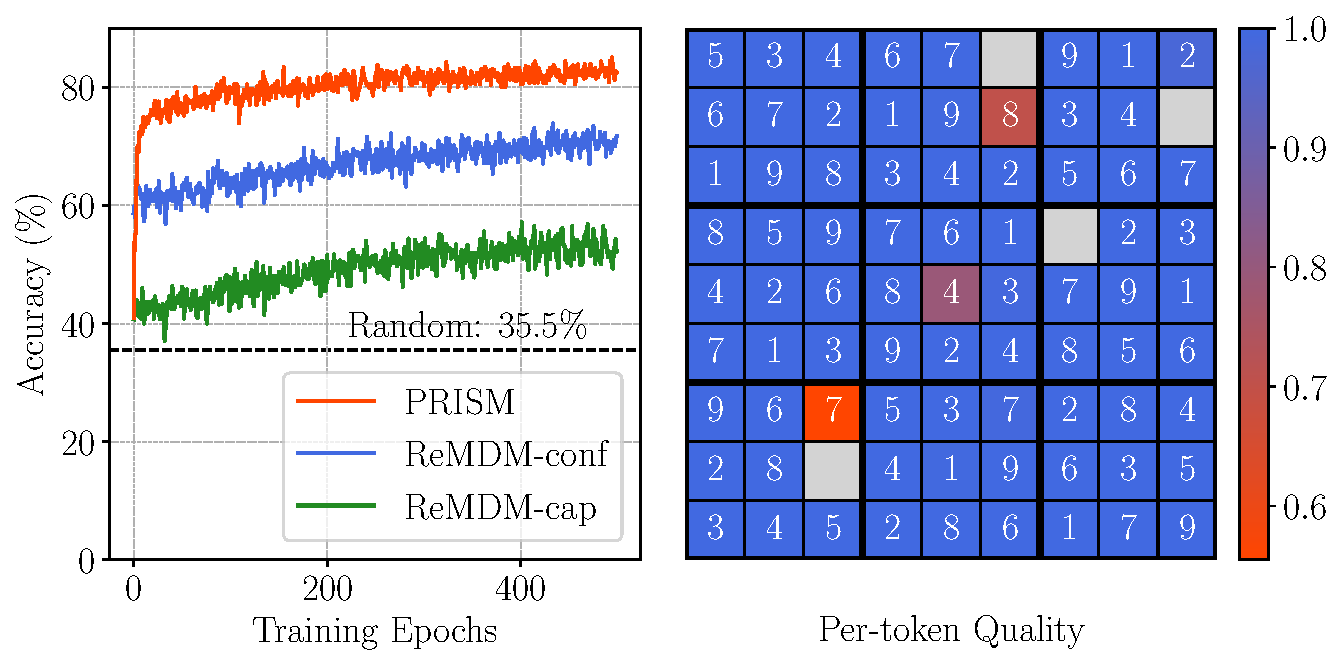
\includegraphics[width=\linewidth]{figs/merged_sudoku_hq.pdf}
    \vspace{-20pt}
    \captionof{figure}{\textbf{Left:} PRISM achieves higher success accuracy on Sudoku puzzles than baselines. (\coloredul{xred}{red line}) \textbf{Right:} PRISM detects the incorrect cells by assigning low per-token quality (\coloredul{xred}{red-colored cells}).}
    \label{fig:sudoku-success-rate_}
\end{minipage}

\textbf{Results.} We evaluate the success rate for the same model across epochs for PRISM and baselines. As shown in Figure~\ref{fig:sudoku-success-rate_}, PRISM achieves progressively higher success rates during fine-tuning (\coloredul{xred}{red line}) and surpasses the baselines. This confirms that the learned per-token quality enables effective self-correction at inference. Notably, PRISM starts to outperform vanilla MDM inference (\coloreddashul{black}{dashed line}) and baselines within only a few epochs, far fewer than the pretraining epochs ($\approx 530$), corroborating our claim of sample efficiency. 

\textbf{Visualization of learned per-token quality.} Figure~\ref{fig:sudoku-success-rate_} further visualizes PRISM's ability to detect incorrect tokens. On the shown board, three digits are misfilled: $(2,6)=8$, $(5,5)=4$, and $(7,3)=7$. The computed per-token quality assigns low scores to these cells (\coloredul{xred}{red}), while other cells attain high scores, nearly $0.99$ (\coloredul{xblue}{blue}), indicating that the fine-tuned model has almost perfectly learned the per-token quality.

\subsection{Unconditional Text Generation} \label{sec:owt}
\textbf{Setup}. We first take a DiT-based MDM with $170$M parameters, using a checkpoint from~\citep{sahoo2024simple}. This MDM is pretrained on the OpenWebText corpus~\citep{Gokaslan2019OpenWeb} with the GPT-2 tokenizer~\citep {radford2019language}, a maximum sequence length $L=1024$, and a total of $262$B tokens. We then attach a lightweight $7$M parameter adapter, one attention layer applied to the final hidden state, and fine-tune it with the PRISM loss on a total $164$M tokens from the same OpenWebText corpus. This fine-tuning is data-efficient, using $\mathbf{1600}\times$ fewer tokens than pretraining.

\textbf{Results.} We then assess the performance of PRISM and baselines on unconditional generation. Our primary metrics are Generative Perplexity and MAUVE \citep{pillutla2021mauve}, which respectively assess per-sequence fluency and distributional similarity between generated samples and the reference distribution. Moreover, given the prior observation~\citep{zheng2024masked} that a sequence with too many redundant tokens can spuriously yield better (i.e., lower) generative perplexity, we also report the entropy as a sanity metric. Following standard evaluation protocols~\citep{pillutla2021mauve, wang2025remasking}, we generate $5000$ samples to compute both metrics, using GPT-2-Large as the reference model. As shown in Figure~\ref{fig:mauve-and-gen-ppl-plot}, PRISM 
outperforms baselines on both metrics (\coloredul{xred}{red lines}) while achieving a comparable entropy, especially in the regime with fewer sampling steps ($N<1024$).

\textbf{Sampling strategy.} 
As sentence diversity is crucial for unconditional generation, we observe that the vanilla PRISM inference from Section~\ref{sec:prism_inference} can degrade diversity. We attribute this to the greedy nature of the token-remasking policy that ranks positions by per-token quality. To mitigate this, we adopt \emph{PRISM-loop}, analogous to ReMDM-loop~\citep{wang2025remasking}: follow PRISM’s remasking scheme and add \emph{loop} steps at $t_N=0$. After obtaining a clean sequence, in a loop, we randomly remask a subset of tokens and unmask them. A full breakdown of the sampling strategy is given in Appendix~\ref{appendix: prism-loop}, ~\ref{Appendix: owt inference ablations}.
\begin{figure}[t]
  \centering
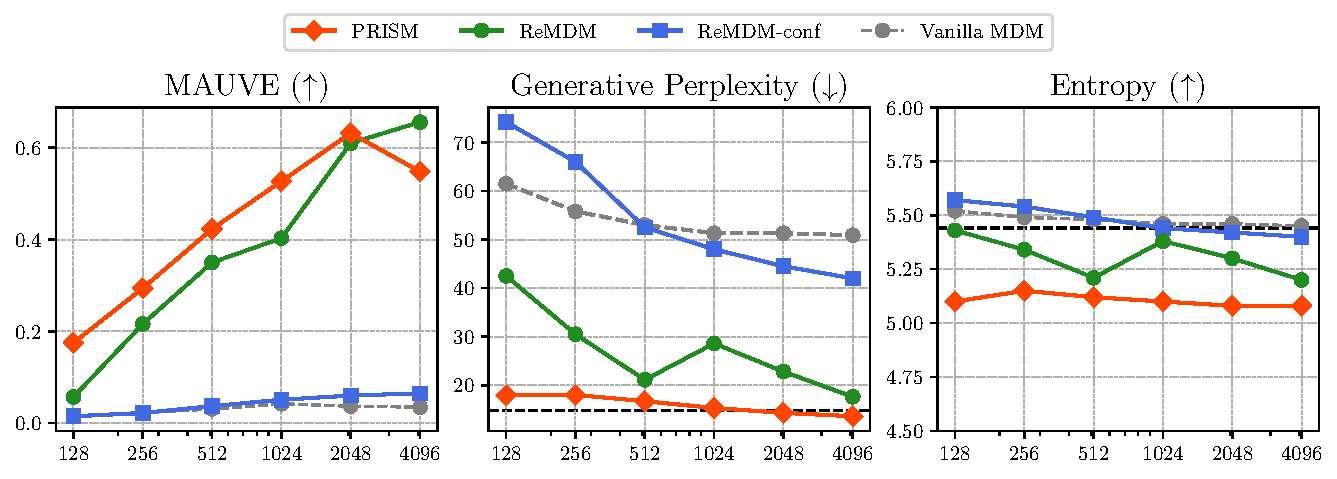
\includegraphics[width=\linewidth, height=0.2\textheight]{figs/gen_quality_owt_plot.pdf}
\caption{\textbf{Unconditional text generation performance.}
\rebuttal{Metrics are evaluated at $\text{NFE} \in \{128, 256, 512, 1024, 2048, 4096\}$; black dashed lines denote validation set references.} PRISM (\coloredul{xred}{red}) outperforms baselines (ReMDM: \coloredul{xgreen}{green}, ReMDM-conf: \coloredul{xblue}{blue}, Vanilla MDM: \coloredul{xgray}{gray}), particularly at lower sampling steps ($N<1024$). \rebuttal{Detailed numerical results are reported in Table~\ref{tab:remdm-exp-owt}.}}


  \label{fig:mauve-and-gen-ppl-plot}
  \vspace{-3.0ex}
\end{figure}

\rebuttal{\textbf{Quantitative analysis.}
To further investigate PRISM’s behavior at a mechanistic level, we evaluate how well its per-token quality scores are calibrated to the desired likelihood.
For partially masked sequences $\mathbf{x}_t$ encountered at inference, we collect per-token quality scores $g_\phi^i(\mathbf{x}_t)$ over all clean positions $i$ and group these tokens into buckets according to the predicted scores.
For each bucket, we then estimate an empirical oracle likelihood and query it by a pretrained model $\theta$; $f_\theta^i(\mathbf{x}_t^i \mid \mathbf{x}_t \oplus \mathbf{m}_i)$ for each $i$. Interestingly, the resulting calibration curves (Figure~\ref{fig:calibration_openweb}) closely follow the queried likelihoods, indicating that $g_\theta^i(\mathbf{x}_t)$ is a well-calibrated estimate of the target posterior, as desired.}

\subsection{Appyling PRISM to $8$B MDM} \label{sec:llada}
\textbf{Setup.} We take LLaDA-$8$B-Instruct~\citep{nie2025large}, an open-sourced $8$B MDM. While freezing the backbone, we add an additional head and a LoRA adapter~\citep{hu2022lora}, for a total of $\approx 250$M trainable parameters. We fine-tune it using the PRISM loss on the opc-sft-stage2~\citep{Huang2024OpenCoderTO} ($0.1$M pairs) for $100$ epochs. Fine-tuning completes in $\approx 30$ hours on $12$ H100 GPUs.


\rebuttal{\textbf{Results.} We evaluate the resulting model in a zero-shot setting on MBPP~\citep{austin2021program} and HumanEval~\citep{chen2021evaluating}, a challenging Python coding benchmarks. As shown in Table~\ref{tab:llada}, PRISM outperforms ReMDM and ReMDM-conf across different numbers of sampling steps. We detail training and inference configurations in Appendix~\ref{appendix: configs},~\ref{appendix:llada}.}

\begin{table*}[h]
    \centering
    \begin{minipage}{0.48\textwidth}
        \centering
        \begin{tabular}{lccc}
            \toprule
            \textbf{Sampling steps} & 256 & 512 & 1024 \\
            \midrule
            PRISM & \textbf{28.0\%} & \textbf{39.0\%} & \textbf{42.7\%}\\
            ReMDM & 26.2\% & 34.8\% & 42.5\%\\
            ReMDM-conf & 25.6\% & 34.1\% & 36.6\%\\
            MDM & 25.6\% & 34.1\% & 36.6\%\\
            \bottomrule
        \end{tabular}
        \caption{\rebuttal{\textbf{HumanEval zero-shot performance.}}}
        \label{tab:llada}
    \end{minipage}
    \hfill
    \begin{minipage}{0.48\textwidth}
        \centering
        \begin{tabular}{lccc}
            \toprule
            \textbf{Sampling steps} & 256 & 512 & 1024 \\
            \midrule
            PRISM & \textbf{21.8\%} & \textbf{29.1\%} & 32.3\%\\
            ReMDM & 19.7\% & 28.5\% & \textbf{32.9\%}\\
            ReMDM-conf & 20.1\% & 29.0\% & 32.5\%\\
            MDM & 18.2\% & 27.8\% & 31.9\%\\
            \bottomrule
        \end{tabular}
        \caption{\textbf{MBPP zero-shot performance.}}
        \label{tab:llada13b}
    \end{minipage}
    \vspace{-0.1in}
\end{table*}

